
\documentclass{article}
\usepackage[utf8]{inputenc}
\usepackage{graphicx}
\usepackage{geometry}
 \geometry{
	 a4paper,
	 total={170mm,257mm},
	 left=20mm,
 	top=20mm,
 }
 
\title{CSIR:Electronically Timing Athletes\\
The Inevitables
}

\author{  
            Peter Rayner\\
            Dawie Pritchard\\
            Drew Langley\\
            Hendrik Jan van der Merwe\\
            Lyle Nel\\
        }


\begin{document}

\maketitle

\includegraphics[width=20cm,height=11cm,keepaspectratio]{group.JPG}

\newpage

\tableofcontents

\newpage


\section{High level description}
For this project we would like to use a raspberry PI or similar device to be able to allow communication between the RFID reader and the tag. As well as using the
device to upload data to a centralized database, this can be done using python and wifi. This database will then be accessed by a website to which the runners will be able to view their individual results and live analysis
on the data for the runner, this will be done using postgreSQL to ensure there are no issues with high usage. This website should be viewable on any device,including mobile.This will be
done using bootstrap,which can dynamically change the site according to the device size.

\section{Proposed Solution}
\subsection{Technologies}
\textbf{RFID Communication} \\
If a Raspberry Pi can be used:  
\begin{itemize}
	\item JEE
	\item JDBC
	\item JPA
	\item WildFly
\end{itemize}
\textbf{Web Portal} 
\begin{itemize}
	\item HTML
	\item CSS / Bootstrap
	\item PHP
	\item JavaScript / JQuery / AJAX
\end{itemize}
\textbf{Database} \\
PostgreSQL

\subsection{Deployment Diagram} 
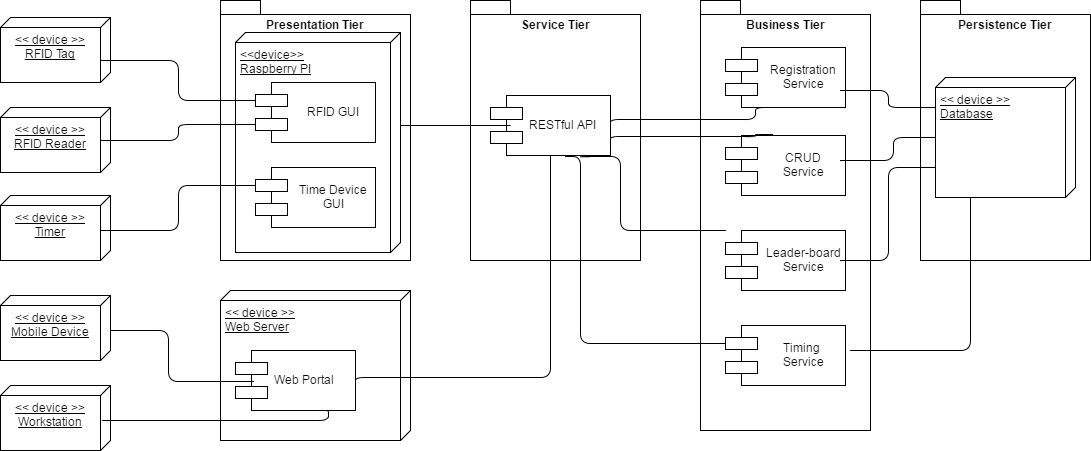
\includegraphics[width=18cm,height=11cm,keepaspectratio]{ETA-Deployment.png}

\section{Development Methodology}
A brief description of the development methodology you intend to follow with particular
reference to team meetings and the role the client will play during the development

\section{Team details}
\subsection{Dawie Pritchard}
\textbf{skills}
\begin{itemize}
 	\item Human Computer Interaction
 	\item Trends, Visual Design 
 	\item Multimedia Specialist
 	\item Computer Scientist
\end {itemize}
\textbf{Technologies known}
\begin{itemize}
	\item C
 	\item C++
 	\item C-Sharp
 	\item CSS
 	\item Bootstrap
 	\item Java
 	\item Python
 	\item Javascript / AngularJS / ExpressJS / NodeJS / JQUERY
 	\item MongoDB / NoSQL
 	\item Php
 	\item SQL
 	\item HTML5
 	\item XML
 \end{itemize}
\textbf{Stengths} 
\begin{itemize}
	\item Front-End
	\item Back-End development
\end{itemize}

\subsection {Peter Rayner}

\textbf{Front-end developer with knowledge of:}
\begin{itemize}
 	\item Artifical Intelligence
 	\item data structures 
 	\item website design 
 	\item databases and human computer interaction(user experience)
 \end{itemize}
\textbf{Knowledge of:}
\begin{itemize}
	\item C++ 
	\item C 
	\item C\# 
	\item Java 
	\item Javascript 
	\item Python 
	\item Assembly 
	\item Angular.js  
	\item Bootstrap
 \end{itemize}
\textbf{Previous industry experience:}\\
Working at Barclays CIB in big data and analytics.
\\
\subsection {Hendrik Jan van der Merwe} 
\textbf{University level knowledge of:}
\begin{itemize}
 	\item Data structures
 	\item Databases
 	\item Human Computer Interaction focussing on User Experience
 	\item System Design
\end{itemize}
\textbf{University Level Experience in:}
\begin{itemize}
	\item C++
	\item C\#
	\item Java
	\item SQL / MySQL
	\item MongoDB
	\item PHP
	\item JavaScript / AJAX / JQuery / NodeJS / ExpressJS
	\item HTML / CSS / Bootstrap
	\item XML
\end{itemize}
\textbf{Strengths:}
\begin{itemize}
	\item Database Design
	\item Backend Development
\end{itemize}

\subsection {Lyle Nel}
\textbf{Qualifications:} \\
I hold a BTEC in software engineering, which included project management as part of the curriculum.
I also hold a BSc in Computer Systems, with relevant subjects such as Software Engineering, Operations management, Knowledge management, Professional development, and Artificial intelligence.\\ \\
\textbf{Digital electronics:} \\
I have worked with Atmel and ARM microprocessors as well as on the arduino platform. In addition I am familiar with most of the common components of a digital circuit including 7400 series and 4000 series integrated circuits. \\ \\
\textbf{Computer Hardware:} \\
I am familiar with all standard consumer hardware and some server hardware. I maintain my own server cluster at home for running experiment. \\ \\
\textbf{Artificial intelligence} \\
I am most experienced in genetic algorithms and I am the author of an open source project that cracks passwords using genetic algorithms. The was one of the top 3 trending projects on github and hackernews a while back. See https://github.com/lyle-nel/siga. In general I am very comfortable with solving problems within the domain of AI. \\ \\
\textbf{Languages} \\
C, C++ including the new C++11, C++14 and C++17 ISO standards, Bash, Python, Javascript, Java, Lisp and Prolog. The language that I am most comfortable with is C++. When I conduct experiment on large datasets I use a mixture between C++, Python and Bash. \\ \\
\textbf{Platforms} \\
I do all of my work in a Linux environment.

\subsection {Drew Langley}
Third year BIS Multimedia student with experience in UX and HCI, animation and 3D modelling, Web design and databases as well as proficiency in programming. I am currently studying networks, software engineering and Artificial Intelligence. \\ \\
\textbf{Languages}
\begin{itemize}
	\item HTML
	\item CSS 
	\item JS / AngularJS / NodeJS / JQuery 
	\item PHP 
	\item SQL
	\item MongoDB
	\item Java 
	\item C++ 
	\item C 
	\item C\# 
	\item Python 
	\item Assembly
\end{itemize}
\textbf{Experience} \\
Designed and developed www.ugandaprohunts.com

\end{document}
